\iffalse
\let\negmedspace\undefined
\let\negthickspace\undefined
\documentclass[journal,12pt,twocolumn]{IEEEtran}
\usepackage{cite}
\usepackage{amsmath,amssymb,amsfonts,amsthm}
\usepackage{algorithmic}
\usepackage{graphicx}
\usepackage{textcomp}
\usepackage{xcolor}
\usepackage{txfonts}
\usepackage{listings}
\usepackage{enumitem}
\usepackage{mathtools}
\usepackage{gensymb}
\usepackage{comment}
\usepackage[breaklinks=true]{hyperref}
\usepackage{tkz-euclide} 
\usepackage{listings}
\usepackage{gvv}                                        
\def\inputGnumericTable{}                                 
\usepackage[latin1]{inputenc}                                
\usepackage{color}                                            
\usepackage{array}                                            
\usepackage{longtable}                                       
\usepackage{calc}                                             
\usepackage{multirow}                                         
\usepackage{hhline}                                           
\usepackage{ifthen}                                           
\usepackage{lscape}
\newtheorem{theorem}{Theorem}[section]
\newtheorem{problem}{Problem}
\newtheorem{proposition}{Proposition}[section]
\newtheorem{lemma}{Lemma}[section]
\newtheorem{corollary}[theorem]{Corollary}
\newtheorem{example}{Example}[section]
\newtheorem{definition}[problem]{Definition}
\newcommand{\BEQA}{\begin{eqnarray}}
\newcommand{\EEQA}{\end{eqnarray}}
\newcommand{\define}{\stackrel{\triangle}{=}}
\theoremstyle{remark}
\newtheorem{rem}{Remark}
\begin{document}
\parindent 0px
\bibliographystyle{IEEEtran}
\title{Assignment CS\_15Q}
\author{EE23BTECH11028 - Kamale Goutham$^{}$% <-this % stops a space
}
\maketitle
\newpage
\bigskip
\section*{Question}
The Lucas sequence $L_{n}$is defined by the recurrence relation:\\
\begin{align*}
    L_{n}=L_{n-1}+L_{n-2}, for n\geq3
\end{align*}
with $L_{1}$=1 and $L_{2}$=3\\
Which one of the option given is TRUE?\\
\begin{enumerate}
    \item $L_{n}=\brak{\frac{1+\sqrt{5}}{2}}^n+\brak{\frac{1-\sqrt{5}}{2}}^n$
    \item $L_{n}=\brak{\frac{1+\sqrt{5}}{2}}^n-\brak{\frac{1-\sqrt{5}}{3}}^n$
    \item $L_{n}=\brak{\frac{1+\sqrt{5}}{2}}^n+\brak{\frac{1-\sqrt{5}}{3}}^n$
    \item $L_{n}=\brak{\frac{1+\sqrt{5}}{2}}^n-\brak{\frac{1-\sqrt{5}}{2}}^n$
\end{enumerate}
\hfill{(GATE 2023 CS 15)}\\
\solution\\
\fi
Initial condition $L_{1}$=1 and $L_{2}$=3
\begin{align}
 L_{n}=L_{n-1}+L_{n-2}
\end{align}
Assume $L_{n+1}=x(n)$\\
\begin{align}
 x(n)=&[x(n-1)+x(n-2)-3]u(n-2)+u(n)+2u(n-1)\\
 X(z)=&z^{-1}(X(z)-1)+z^{-2}X(z)-3\frac{z^{-2}}{1-z^{-1}}+\frac{1}{1-z^{-1}}+2\frac{z^{-1}}{1-z^{-1}}\\
 X(z)&(1-z^{-1}-z^{-2})(1-z^{-1})=1+z^{-1}-2z^{-2}\\
 X(z)&=\frac{1+z^{-1}-2z^{-2}}{(1-z^{-1}-z^{-2})(1-z^{-1})}\\
 X(z)&=\frac{A}{1-z^{-1}}+\frac{B}{1-\alpha z^{-1}}+\frac{C}{1-\beta z^{-1}}
 \end{align}
 Where, $\alpha$ = $\dfrac{1 +\sqrt{5}}{2}$ and $\beta$ = $\dfrac{1 -\sqrt{5}}{2}$ \\
 
	\vspace{0.4cm}
 using partial fractions,
 \begin{align}
     X(z)=\frac{\alpha+2}{(\alpha-\beta)(1-\alpha z^{-1})}+\frac{\beta+2}{(\beta-\alpha)(1-\beta z^{-1})}
 \end{align}
 
	$a^n u(n)$
	$\xleftarrow[]{\hspace{0.4cm}{\mathcal{Z}}\hspace{0.1cm}}\xrightarrow[]{}$
	$\dfrac{1}{1 - a z^{-1}}$ \hspace{0.2cm} $\lvert \hspace{0.1cm} z \hspace{0.1cm}\rvert \hspace{0.1cm} \textgreater \hspace{0.1cm} \lvert \hspace{0.1cm} a \hspace{0.1cm} \rvert$
	
	\vspace{0.4cm}
	
	Substituting this result,
	
	\vspace{-0.5cm}
	
	\begin{align}
		x(n) &= \dfrac{\alpha+2}{(\alpha - \beta)} (\alpha^n u(n)) - \dfrac{\beta+2}{(\alpha - \beta)} (\beta^n u(n))\\
	    x(n) &= \dfrac{(5+\sqrt{5})(1 + \sqrt{5})^{n} - (5-\sqrt{5})(1 - \sqrt{5})^{n} }{2^{n+1} \sqrt{5}} u(n)\\
    	x(n) &= \dfrac{(1 + \sqrt{5})^{n+1} +(1 - \sqrt{5})^{n+1} }{2^{n+1}} u(n)
    \end{align}
$\therefore$ $L_{n} =\brak{\frac{1+\sqrt{5}}{2}}^n+\brak{\frac{1-\sqrt{5}}{2}}^n$
option 1 is correct.
\newpage
\begin{figure}[h]
  \centering
  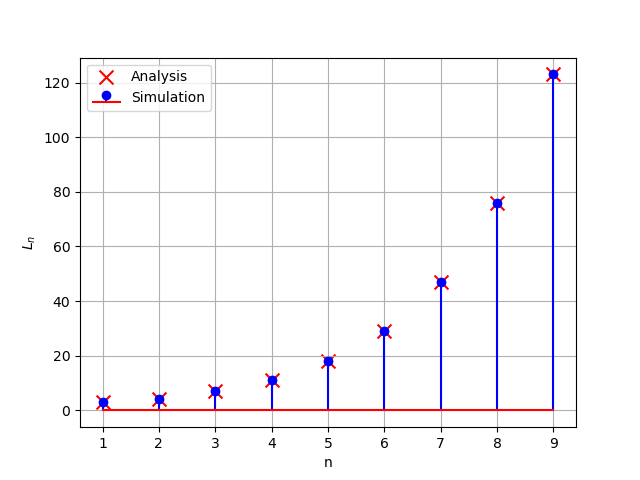
\includegraphics[width=\columnwidth]{2023/CS/15/figs/fig1.png}
  \caption{$L_{n}=\brak{\frac{1+\sqrt{5}}{2}}^n+\brak{\frac{1-\sqrt{5}}{2}}^n$}
  \label{fig:graph}
\end{figure}
